\section{Memory pipeline}
The current



\subsection{Camera to Xavier}
The first step in the memory pipeline is to move the image buffers from the camera to the \jx.
As this link is the current bottleneck of the whole pipeline, it is important to optimize the performance as much as possible.

Firtsly, to get the best possible network performance on the \jx, several network configurations were performed as discussed Section\ref{sec:network_configuration}.

Secondly, the \cams have a multitude of differend settings that can be configured to optimize the performance.
One important step is to

The \cams have an internal Image buffer of 128MB, which is used to store the image data before it is sent to the \jx.
With 10-bit resolution per image the


\begin{align}
    \frac{128*1000000*8}{2048*2448*10}
\end{align}

\subsection{Image buffer to Device Memory}
Pinned host to host,
Pinned host to device,
Device host to device, -> nsys

\subsubsection{Device to Shared}
This is discussed thuroughly in Section



\begin{figure}[H]
    \centering
    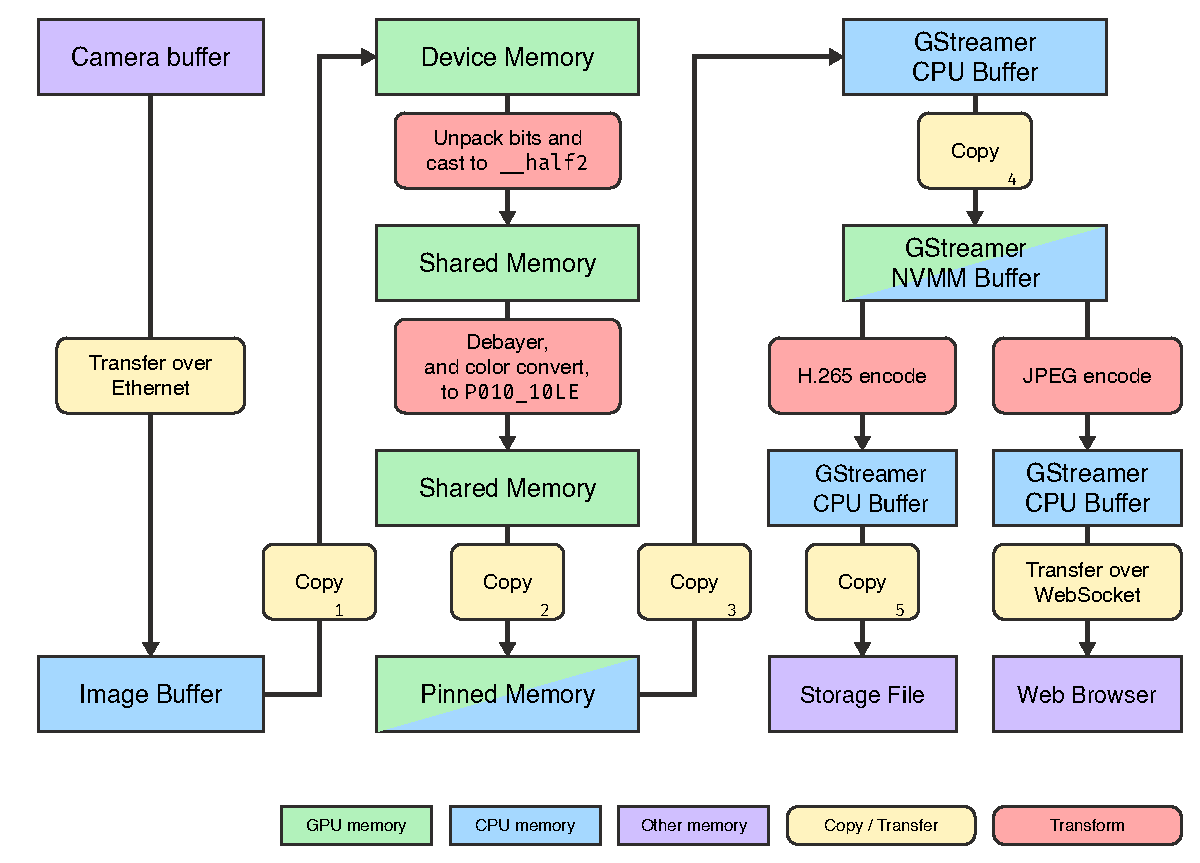
\includegraphics[width=\textwidth]{figures/memory_pipeline/current.pdf}
    \caption{Overview of the memory movement in the current pipeline.}
    \label{fig:pipeline_current}
\end{figure}

\subsection{Challenges and future work}
There are two major potential improvements in the current pipeline that remain

\subsubsection{Store image buffers directly in GPU accessable memory}
The first potential improvement is to store the image buffers directly in GPU accessable memory, as it will remove the redundant first copy operation in Figure \ref{fig:pipeline_current}.
This improvement relies on \lucid changing their \gls{api} as the current \gls{api} does not support this and the source code is not available.
I have communicated with a \lucid employee over email, and he said that they will looking into adding this feature in the future \cite{martensRe17896Use2023}.
After some discussion on how this could be implemented we came to the conclusion that a clean way would be have an optional argument that would make the \gls{api} use Pinned Memory instead of regular Pageable host memory.
Another more modular approach I sugessted is to allow the user to pass in pointers to where the images should be stored, enabling the use of any tyupe of \gls{cpu} accessable memory.
As of today the engenering department at \lucid has not yes implemented any of these features, but hopefully they will be implemented in the future.

\subsubsection{Better integration with GStreamer}
Use \gls{pyds} in the future hopefully.

\begin{figure}[H]
    \centering
    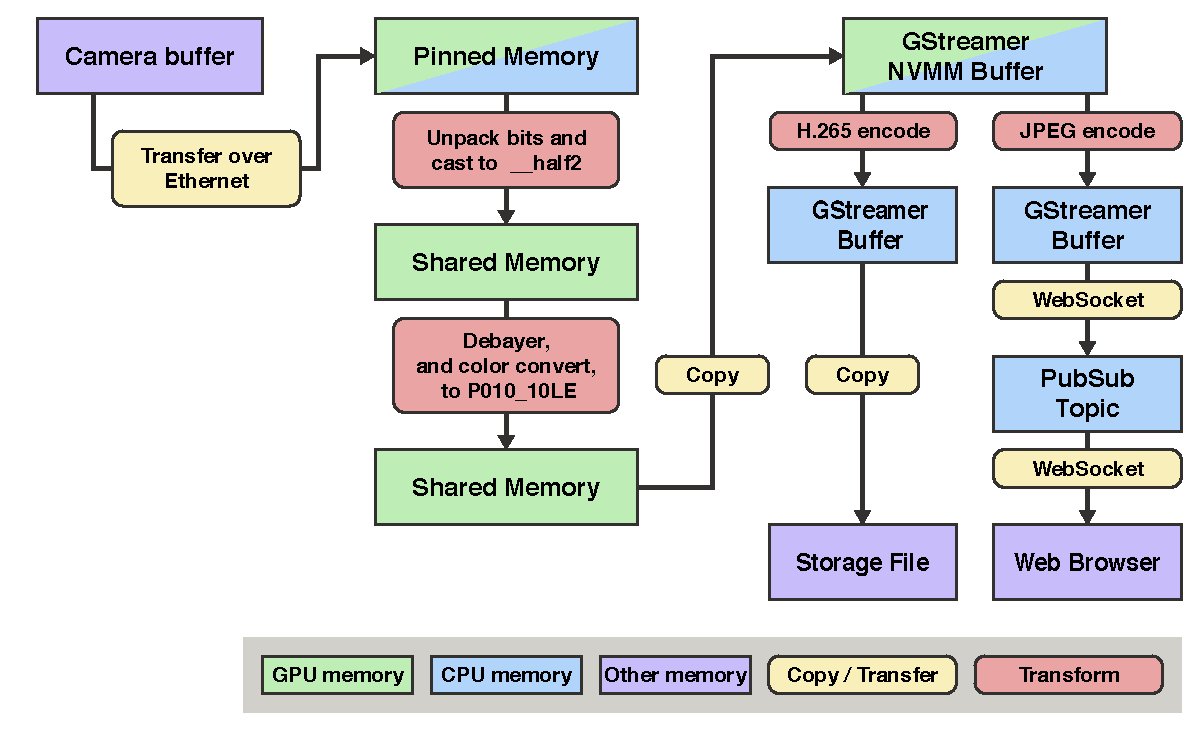
\includegraphics[width=\textwidth]{figures/memory_pipeline/optimal.pdf}
    \caption{Overview of the memory pipeline}
    \label{fig:pipeline_optimal}
\end{figure}